\documentclass[tikz,border=12pt]{standalone}
\usepackage[T1]{fontenc}
\usepackage{mathpazo}
\usepackage{amsmath,amssymb}
\usetikzlibrary{arrows.meta, positioning, calc}

\definecolor{stblue}{HTML}{7B97AD}
\definecolor{rwgold}{HTML}{B8995E}
\definecolor{sage}{HTML}{7A9A7E}
\definecolor{dkbrown}{HTML}{3D3530}
\definecolor{wmgray}{HTML}{7B7067}
\definecolor{cream}{HTML}{F9F6F0}
\definecolor{border}{HTML}{D4C9B8}
\definecolor{terracotta}{HTML}{C47A6A}

\begin{document}
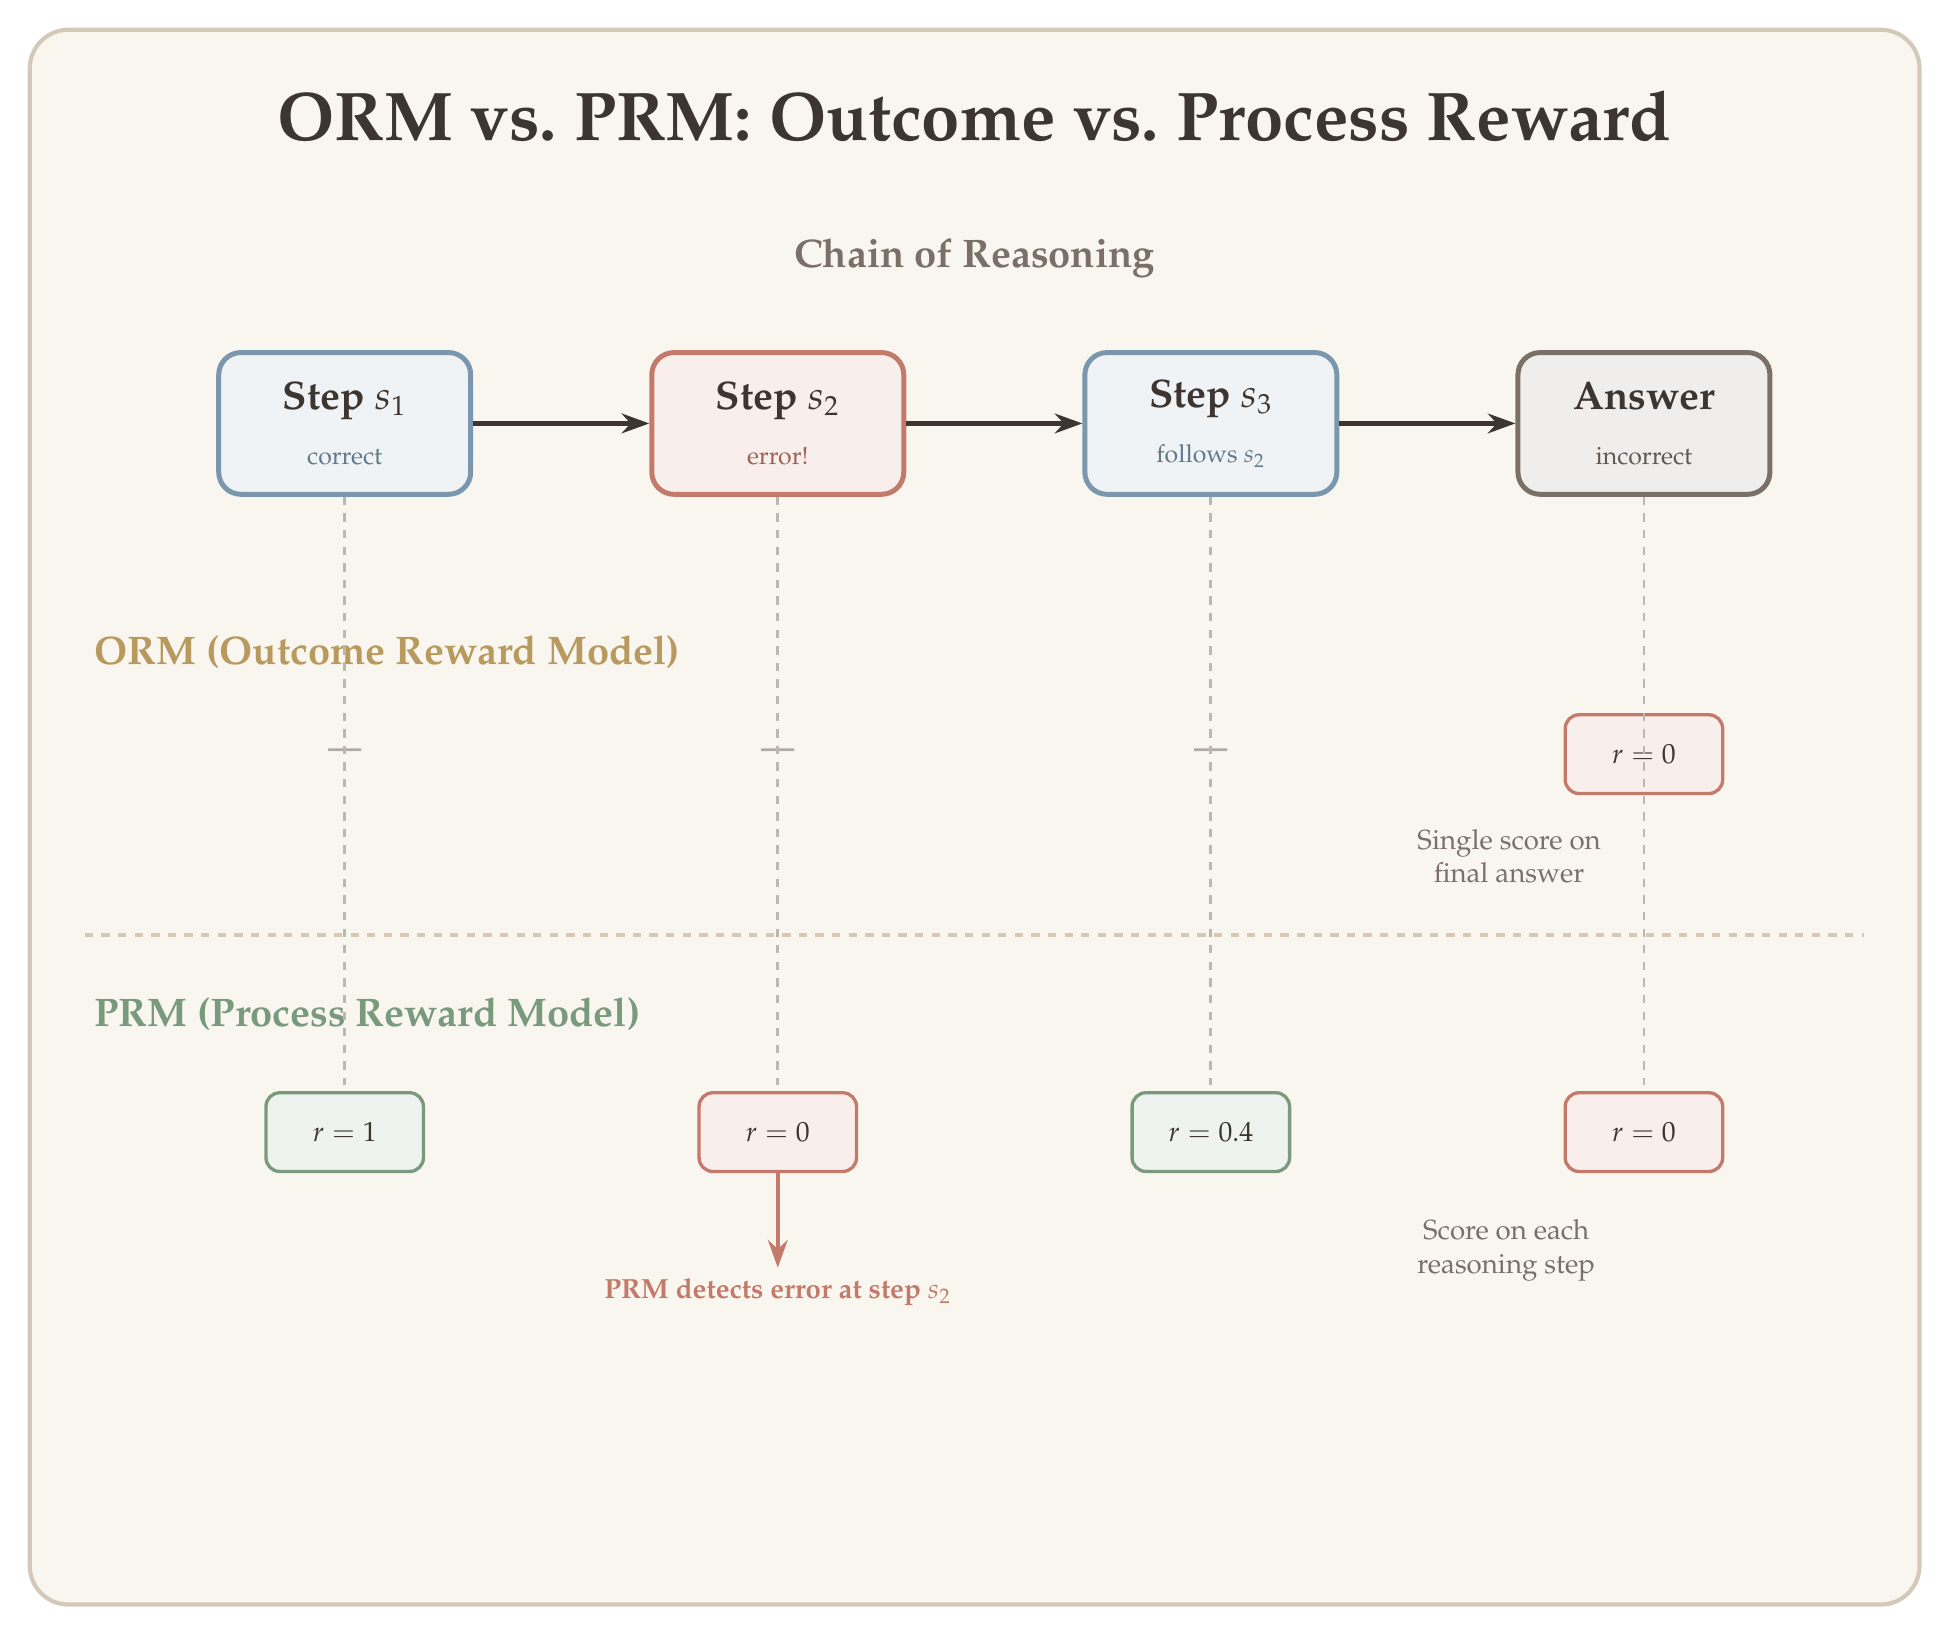
\begin{tikzpicture}[
  >={Stealth[length=3.5mm, width=2.5mm]},
  stepbox/.style 2 args={
    draw=#1, line width=1.8pt, fill=#1!12, rounded corners=8pt,
    minimum width=32mm, minimum height=18mm, font=\Large,
    text=dkbrown, align=center, inner sep=5pt
  },
  scoretag/.style 2 args={
    draw=#1, line width=1.2pt, fill=#1!12, rounded corners=5pt,
    minimum width=20mm, minimum height=10mm, font=\normalsize,
    text=dkbrown, align=center, inner sep=3pt
  },
  dashscore/.style={
    font=\large, text=wmgray!60, align=center
  },
  arr/.style={->, line width=2pt, dkbrown},
  note/.style={font=\normalsize, text=wmgray, align=center},
]

% Background
\fill[cream, rounded corners=14pt] (-1,-2.5) rectangle (23,17.5);
\draw[border, rounded corners=14pt, line width=1.5pt] (-1,-2.5) rectangle (23,17.5);

% Title
\node[font=\Huge\bfseries, text=dkbrown] at (11,16.4)
  {ORM vs.\ PRM: Outcome vs.\ Process Reward};

% =============================================
% Chain of Reasoning (top)
% =============================================
\node[font=\Large\bfseries, text=wmgray] at (11,14.6)
  {Chain of Reasoning};

% Step boxes
\node[stepbox={stblue}{}] (s1) at (3,12.5)
  {\textbf{Step $s_1$}\\[2pt]
   \small\color{stblue!80!black} correct};

\node[stepbox={terracotta}{}] (s2) at (8.5,12.5)
  {\textbf{Step $s_2$}\\[2pt]
   \small\color{terracotta!80!black} error!};

\node[stepbox={stblue}{}] (s3) at (14,12.5)
  {\textbf{Step $s_3$}\\[2pt]
   \small\color{stblue!80!black} follows $s_2$};

\node[stepbox={wmgray}{}] (ans) at (19.5,12.5)
  {\textbf{Answer}\\[2pt]
   \small\color{wmgray!80!black} incorrect};

% Arrows between steps
\draw[arr] (s1.east) -- (s2.west);
\draw[arr] (s2.east) -- (s3.west);
\draw[arr] (s3.east) -- (ans.west);

% =============================================
% ORM Section (middle)
% =============================================
\node[font=\Large\bfseries, text=rwgold, anchor=west] at (-0.3,9.6)
  {ORM (Outcome Reward Model)};

% Dashes under steps (no per-step scores)
\node[dashscore] at (3, 8.3) {\textbf{---}};
\node[dashscore] at (8.5, 8.3) {\textbf{---}};
\node[dashscore] at (14, 8.3) {\textbf{---}};

% Single score under Answer
\node[scoretag={terracotta}{}] (orm-score) at (19.5, 8.3)
  {\textbf{$r = 0$}};

% Annotation
\node[note, anchor=west] at (16.5, 7.0)
  {Single score on\\final answer};

% =============================================
% Divider
% =============================================
\draw[dashed, line width=1.5pt, border] (-0.3,6.0) -- (22.3,6.0);

% =============================================
% PRM Section (bottom)
% =============================================
\node[font=\Large\bfseries, text=sage, anchor=west] at (-0.3,5.0)
  {PRM (Process Reward Model)};

% Per-step scores
\node[scoretag={sage}{}] (prm1) at (3, 3.5)
  {\textbf{$r = 1$}};

\node[scoretag={terracotta}{}] (prm2) at (8.5, 3.5)
  {\textbf{$r = 0$}};

\node[scoretag={sage}{}] (prm3) at (14, 3.5)
  {\textbf{$r = 0.4$}};

\node[scoretag={terracotta}{}] (prm4) at (19.5, 3.5)
  {\textbf{$r = 0$}};

% Dashed lines connecting steps to PRM scores
\draw[dashed, line width=1pt, wmgray!50] (s1.south) -- ++(0,-1.5) -- (3, 4.1);
\draw[dashed, line width=1pt, wmgray!50] (s2.south) -- ++(0,-1.5) -- (8.5, 4.1);
\draw[dashed, line width=1pt, wmgray!50] (s3.south) -- ++(0,-1.5) -- (14, 4.1);
\draw[dashed, line width=1pt, wmgray!50] (ans.south) -- ++(0,-1.5) -- (19.5, 4.1);

% Arrow from s2 PRM score down to annotation
\draw[->, line width=1.5pt, terracotta] (prm2.south) -- ++(0,-1.2)
  node[below, font=\normalsize\bfseries, text=terracotta, align=center]
  {PRM detects error at step $s_2$};

% Side annotation
\node[note, anchor=west] at (16.5, 2.0)
  {Score on each\\reasoning step};

\end{tikzpicture}
\end{document}
